\section{Case Study: Dynamic Throwing \\ with a 7-DoF Robot Arm}

In this section, we demonstrate our method on a dynamic throwing task with a 7‑DoF Franka Panda arm, a challenging scenario that requires solving a kinodynamic optimization with nonlinear objectives and tight constraints.  
The solution depends heavily on initial conditions and is computationally expensive, making it ideal to showcase the benefits of our approach.

\textbf{Task setup.}  
As shown in Fig.~\ref{fig:target_position}, the task parameter is the target box position $\tau = (r\cos\theta, r\sin\theta, h)\in\mathbb{R}^3$ from the robot base.  
We exploit rotational symmetry by fixing $\theta=0$, since nonzero $\theta$ can be handled by rotating the first joint.  
Therefore, the task parameter space for training models is 
\[
{\cal T} = \{(r,0,h)\mid r\!\in\![1.1,2.0],\ h\!\in\![0.0,0.3]\},
\]
excluding close targets where throwing is unnecessary.  
The throwing time $\eta \in [0,T]$ with $T=5$ is an additional variable, and the release phase is $(q(\eta),\dot q(\eta))$.  
We assume the object is released instantaneously at time~$\eta$, with the velocity determined by the end‑effector at that instant.

\begin{figure}[!t]
    \centering
    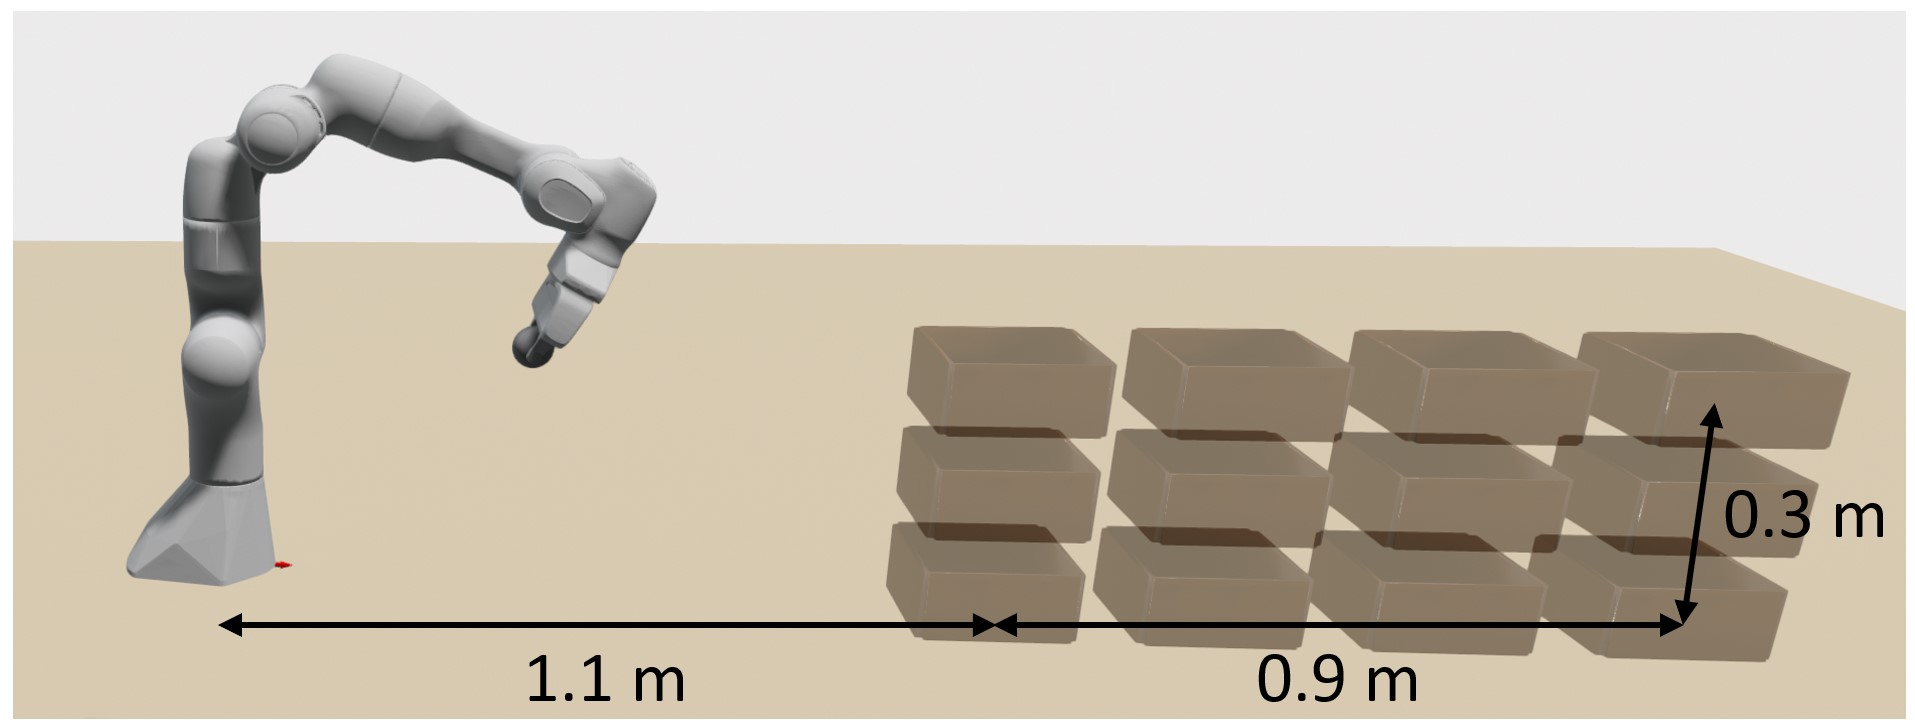
\includegraphics[width=0.9\linewidth]{task.jpg}
    \caption{Task parameter space ${\cal T}$, a set of positions of the target box.}
    \label{fig:target_position}
\end{figure}

\textbf{Objective.}  
Using free‑fall dynamics, the landing position is computed and the objective is defined as
\begin{equation}
J(q(\cdot),\eta;\tau) = J_{\rm task}(q(\cdot),\eta;\tau) + w_1 \int_0^T \|\dddot q(t)\|^2 dt,
\end{equation}
where $J_{\rm task}$ is the squared position error when the thrown object crosses the target box’s $z$‑level (height).


\textbf{Constraints.}  
We enforce limits on joint position, velocity, acceleration, and jerk; end‑effector velocity limits; torque limits derived from the dynamics; and self‑collision margins using capsule models.  
All constraints are expressed as $C(q,\dot q,\ddot q,\dddot q)\le0$, with added safety margins.  
We use the standard limits of the Franka Emika Panda, except that the end‑effector velocity limits are doubled to enable throws of up to 2\,m (in simulation).

\textbf{Implementation.}  
We weight trajectory errors by $c(t)=\exp\!\big(-4(t-\eta)^2\big)$ in (\ref{eq:reconloss}) to achieve higher accuracy near the throwing time.
In the basis model (\ref{eq:lbfnn}), $N_b=100$.  
All modules use fully connected networks with GELU activations (4-6 layers, 1024 nodes).  
The subset of task parameters for optimization is
\[
{\cal T}_s=\{(r,0,h)\mid r\!\in\!\{1.1,\dots,2.0\},\ h\!\in\!\{0.0,0.1,0.2,0.3\}\}.
\]
All kinematics, dynamics, and constraints are implemented in PyTorch. The latent ODE~(\ref{eq:lsode}) is integrated using the Euler method with step size $ds=0.1$, providing a good balance between accuracy and speed.


\subsection{Data Collection via Trajectory Optimizations} 
\label{sec:dcto}



We use the parametric trajectory model $q_{q_0,q_T,w}$ (\ref{eq:parmetric_model}) with $B=20$, so $w \in \mathbb{R}^{20 \times 7}$.  
The optimization variable $w$ is initialized to zero, and $\eta$ is set to $2$.  
To randomly initialize $q_0$ and $q_T$ within joint limits, we sample $v_0,v_T \in \mathbb{R}^7$ from a standard Gaussian, apply the sigmoid function, and scale them by the joint limits.  
Empirically, initialization in the vicinity of the origin leads to improved performance compared to uniform sampling, since extreme initial configurations can adversely affect convergence during optimization.


\begin{figure}[!t]
    \centering
    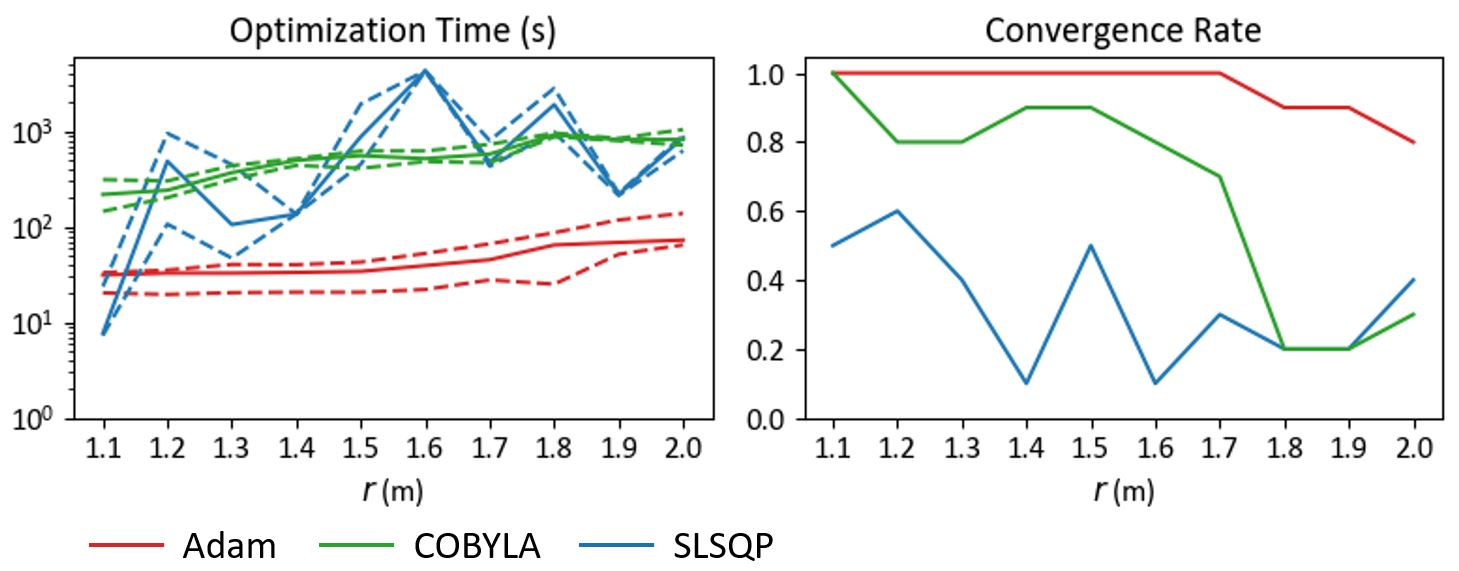
\includegraphics[width=\linewidth]{opt_graph.jpg}
    \caption{Quartiles of the optimization times and convergence rates as functions of \( r \in [1.1, 2.0] \), where the target box position is \(\tau = (r, 0, 0)\). The quartiles are computed using only the successful cases from 10 optimization attempts.}
    \label{fig:opt_graph}
\end{figure}

We first compare trajectory optimizers SLSQP~\cite{kraft1988software}, COBYLA~\cite{powell1994direct}, and Adam~\cite{kingma2014adam} by computation time and success rate.  
For Adam, constraints are added to the objective via a ReLU penalty.  
Optimization stops when constraints meet thresholds and position error $<0.01$, or after 10,000 iterations.  
Fig.~\ref{fig:opt_graph} shows that all solvers take over 10 s and are sensitive to initialization; Adam performs best but still fails beyond $r=1.7$, highlighting the problem’s complexity and the challenge of achieving sub‑second planning.



\begin{figure}[!t]
    \centering
    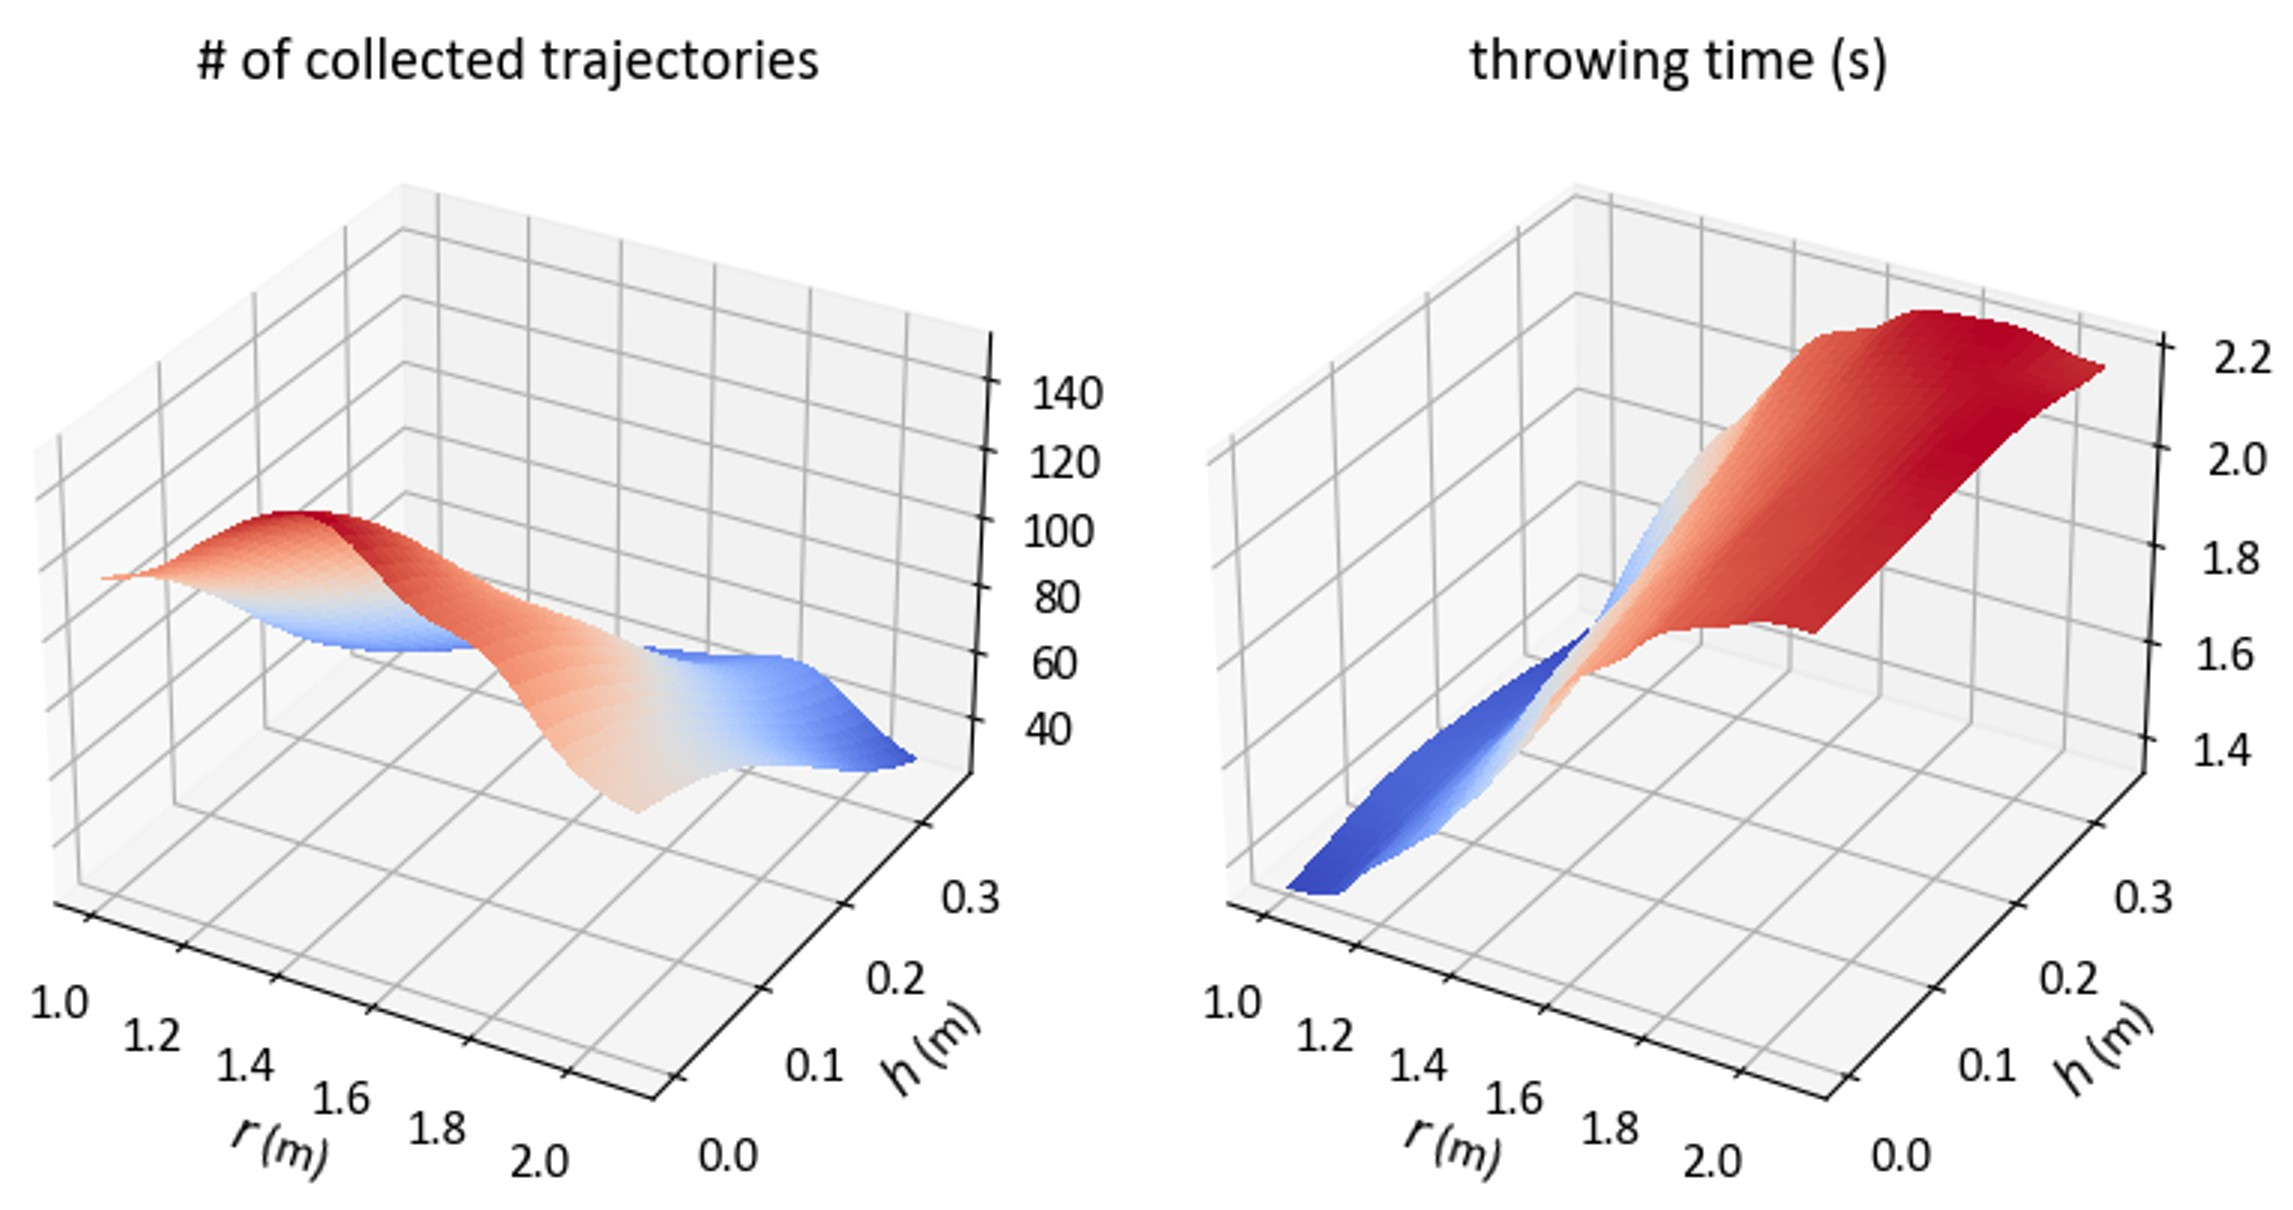
\includegraphics[width=\linewidth]{data_stat.jpg}
    \caption{The number of collected trajectories and throwing times as functions of $r$ and $h$, where the target box position is $\tau = (r, 0, h)$.}
    \label{fig:datastat.}
\end{figure}

We collect trajectories by repeatedly solving the optimization with the Adam optimizer.  
For each $\tau \in {\cal T}_s$, 300 trajectories are optimized, yielding 12,000 candidates across 40 parameters.  
After excluding failure cases, 3,523 valid trajectories remain.  
Fig.~\ref{fig:datastat.} ({\it Left}) shows their distribution over task parameters, and Fig.~\ref{fig:datastat.} ({\it Right}) shows the mean throwing time $\eta$ as a function of the task parameters.  
As expected, fewer trajectories are obtained and $\eta$ increases as the target distance grows.




\subsection{Comparisons of Planning Performance}

\begin{table*}[!t]
\tiny
\centering    
\caption{Average success rates, position error, and various constraint satisfaction rates. Computations are performed using an AMD Milan 2.8 GHz 8-core processor for trajectory optimizations and AMD Ryzen 9 5900x 12-Core Processor and NVIDIA GeForce RTX 3090 for motion manifold primitives.}
\label{tab:main_table}
\begin{tabular}{lcccccccccccccccccccc}
\toprule
& \multicolumn{9}{c}{Seen Task Parameter} & \multicolumn{9}{c}{Unseen Task Parameter}  & \multirow{2}{*}{$\#$ Traj.} & \multirow{2}{*}{Time} \\ 
\cmidrule(lr){2-10} \cmidrule(lr){11-19}
&  SR & Error & JL & JVL & JAL & JJL & CVL & JTL & COL & SR & Error & JL & JVL & JAL & JJL & CVL & JTL & COL &  &\\ 
\midrule 
TO (Adam)~\cite{kingma2014adam} & 97 & 0.01 & 100 & 100 & 100 & 100 & 100 & 100 & 100 & 100 & 0.01 & 100 & 100 & 100 & 100 & 100 & 100 & 100 & 1 & 10 $\sim$ 100 s \\
TO (SLSQP)~\cite{kraft1988software} & 33 & 0.01 & 100 & 100 & 100 & 100 & 100 & 100 & 100 & 100 & 0.01 & 100 & 100 & 100 & 100  & 100 & 100 & 100 & 1 & 10 $\sim$ 3000 s \\
TO (COBYLA)~\cite{powell1994direct} & 66 & 0.01 & 100 & 100 & 100 & 100 & 100 & 100 & 100 & 100 & 0.01 & 100 & 100 & 100 & 100 & 100 & 100 & 100 & 1 & 100 $\sim$ 1000 s \\
MMP~\cite{lee2023equivariant} & 1.05 & 0.53 & 0.95 & 0.0 & 0.0 & 0.0 & 0.0 & 0.0 & 92.6 & 0.81 & 0.53 & 96.4 & 0.0 & 0.0 & 0.0 & 0.0 & 0.0 & 94.4 & 100 & 0.003s \\
MMFP~\cite{lee2025motion} & 77.4 & 0.05 & 97.7 & 0.0 & 0.0 & 0.0 & 0.0 & 0.0 & 99.0 & 15.0 & 0.15 & 0.0 & 0.0 & 0.0 & 0.0 & 0.0 & 0.0 & 99.3 & 100 & 0.011s\\
DMMFP & 17.5 & 0.18 & 99.2 & 72.5 & 25.9 & 100 & 89.5 & 64.7 & 98.6 & 4.96 & 0.26 & 99.4 & 79.5 & 32.7 & 100 & 93.1 & 87.4 & 98.4 & 100 & 0.012s\\
DMMFP + TMO & 95.8 & 0.01 & 100 & 93.0 & 99.9 & 100 & 99.9 & 100 & 100 & 94.1 & 0.02 & 100 & 80 & 98.2 & 100 & 100 & 100 & 100 & 100 & 0.012s \\ 
DMMFP + TMO + RS & 100 & 0.01 & 100 & 100 & 100 & 100 & 100 & 100 & 100 & 100 & 0.01 & 100 & 100 & 100 & 100 & 100 & 100 & 100 & 91 & 0.227s  \\ 
\bottomrule
\end{tabular}
\end{table*}

\begin{figure*}[!t]
    \centering
    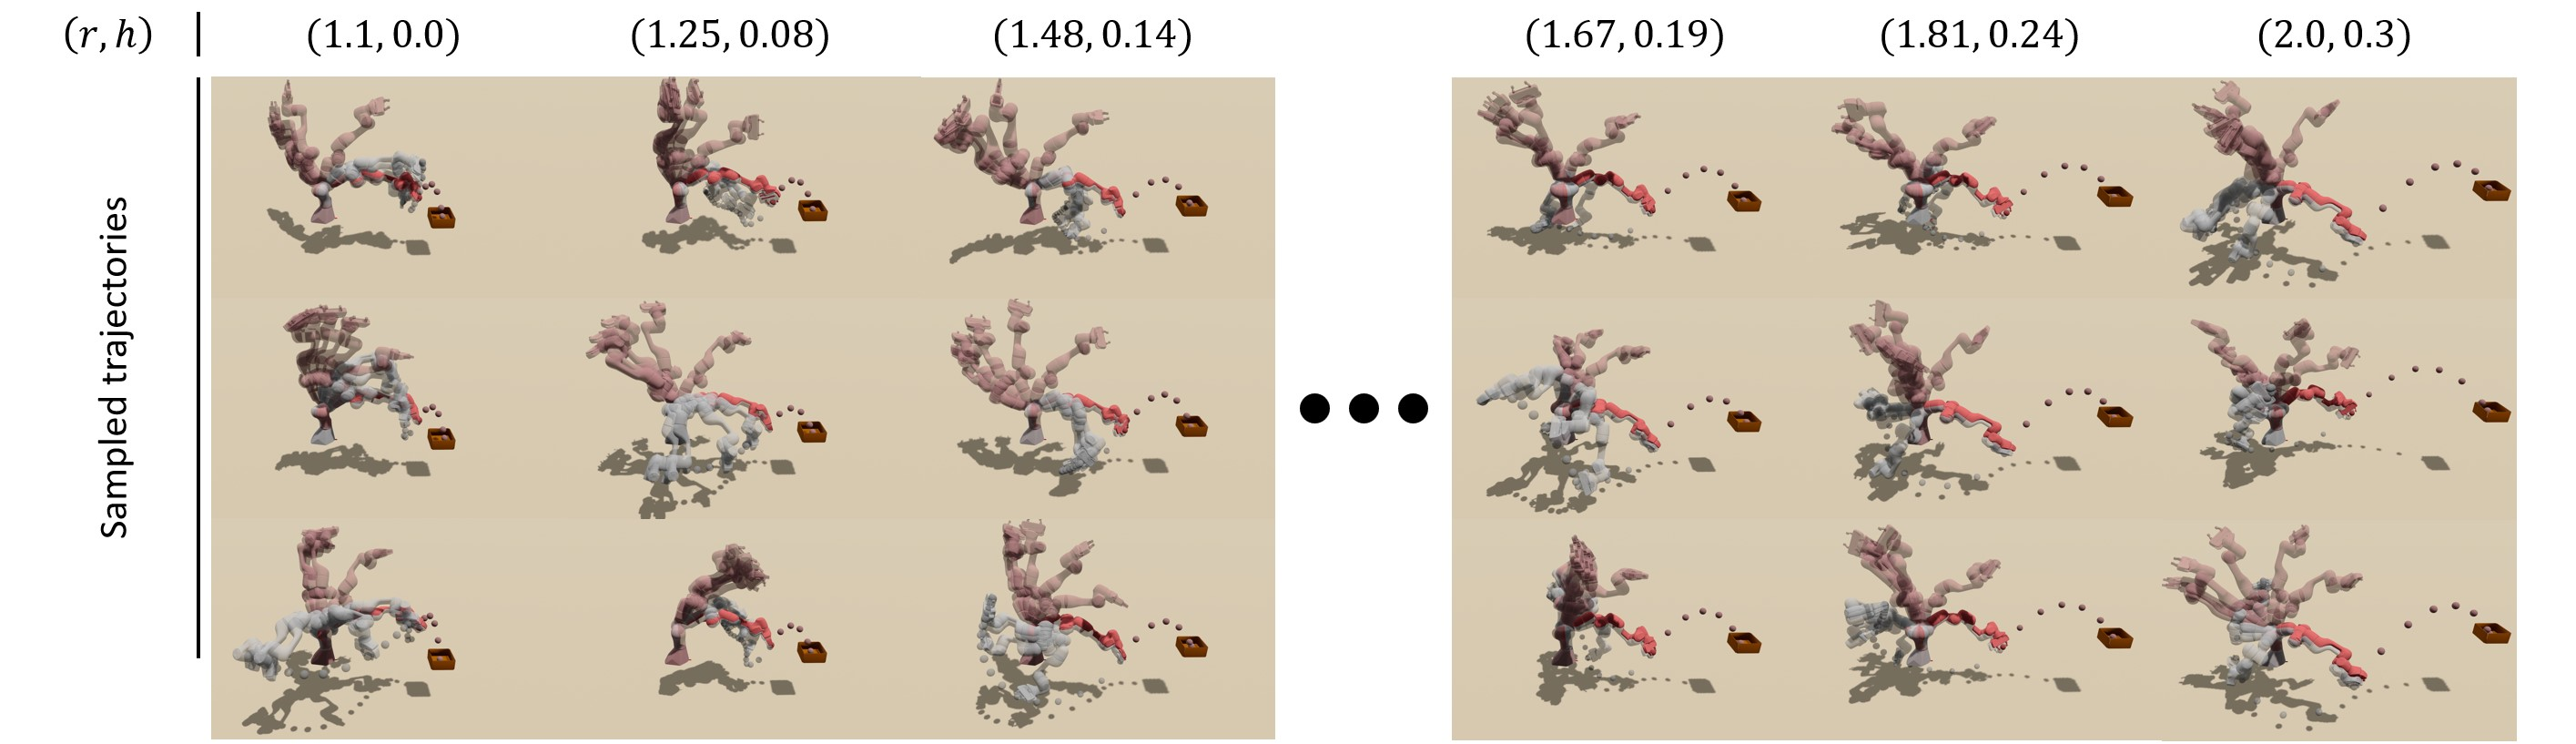
\includegraphics[width=\textwidth]{results1.jpg}
    \caption{Examples of diverse generated trajectories by {\it Differentiable Motion Manifold Primitives (DMMFP) + Trajectory Manifold Optimization (TMO) + Rejection Sampling (RS)} for various task parameters $\tau=(r,0,h)$. The moment of the throw is depicted in deep red, preceded by gray and followed by transparent red.}
    \label{fig:results1}
\end{figure*}

\begin{figure*}[!t]
    \centering
    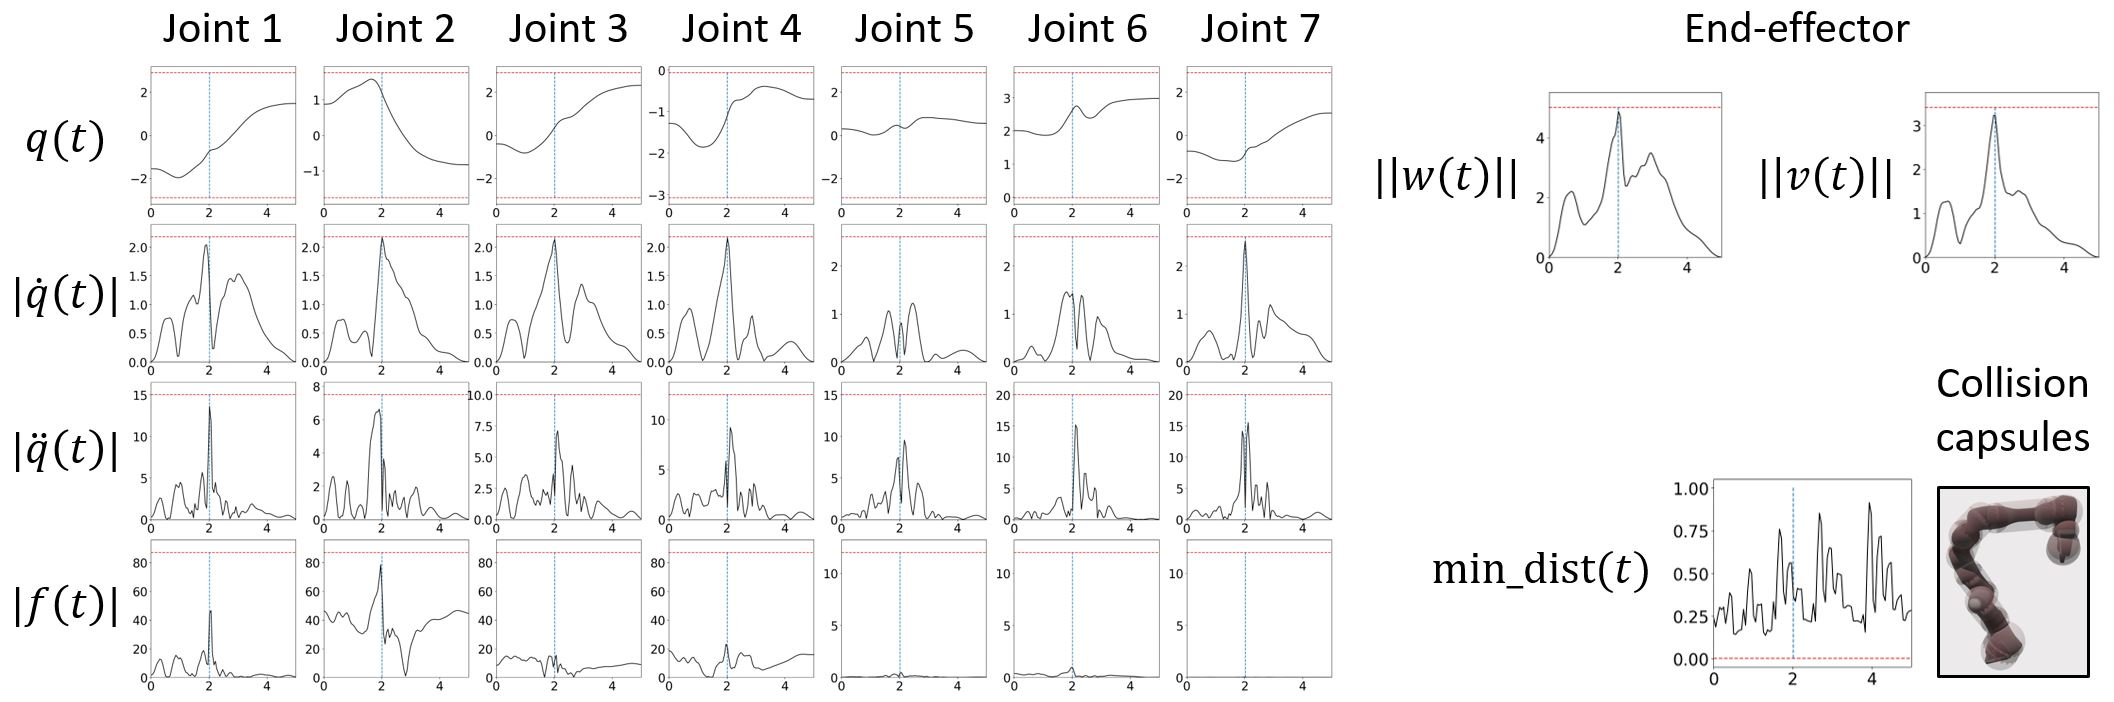
\includegraphics[width=0.8\textwidth]{graph.jpg}
    \caption{Trajectories of joint $q(t)$, joint velocity $\dot{q}(t)$, joint acceleration $\ddot{q}(t)$, joint torque $f(t)$, end-effector angular velocity $w(t)$, end-effector linear velocity $v(t)$, and minimum distance between links ${\rm min}\_{\rm dist}(t)$ for an example throwing motion generated by {\it DMMFP + TMO + RS} given the task parameter $\tau=(2.0, 0, 0.3)$. The limit values are visualized as red horizontal lines. The moment of throw is marked in blue vertical lines.}
    \label{fig:results2}
\end{figure*}


In this section, we compare {\it Trajectory Optimization (TO)} with the parametric curve models detailed in section~\ref{sec:dcto}, and motion manifold-based methods: {\it Motion Manifold Primitives (MMP)} with a Gaussian mixture prior~\cite{lee2023equivariant}, {\it Motion Manifold Flow Primitives (MMFP)}~\cite{lee2025motion}, and our {\it Differentiable Motion Manifold Flow Primitives (DMMFP)}, each of which is trained with a $32$-dimensional latent space. To train MMP, MMFP, and DMMFP, we use the same trajectory dataset collected via trajectory optimizations in section~\ref{sec:dcto}. We fine-tune the DMMFP using {\it Trajectory Manifold Optimization (TMO)} introduced in section~\ref{sec:D}, and denote it by ${\it DMMFP + TMO}$. 
Some generated trajectories by DMMFP + TMO may not meet the required constraints or task goals. Therefore, we use {\it Rejection Sampling (RS)} to exclude non-compliant samples, denoted by {\it DMMFP + TMO + RS}, although this step necessitates extra computation to verify the feasibility of the trajectories.


TABLE~\ref{tab:main_table} presents the averaged Success Rate (SR) -- a motion \((q(t), \eta)\) is deemed successful if the position error is less than 0.04 --, Position Error (Error) in meter scale, and Constraint Satisfaction Rates on Joint Limits (JL), Joint Velocity Limits (JVL), Joint Acceleration Limits (JAL), Joint Jerk Limits (JJL), Cartesian Velocity Limits (CVL), Joint Torque Limits (JTL), and Self-Collisions (COL).
A trajectory is considered to satisfy a constraint if it meets the requirement at every time \(t \in [0,T]\) along the trajectory. 
These metrics are computed using both seen task parameters $\tau \in {\cal T}_s$ and unseen test task parameters $\tau \in \{(r,0,h)| r \in \{1.15, 1.25, \ldots, 1.95\}, h \in \{0.05, 0.15, 0.25 \} \}$.
The number of trajectories generated simultaneously is reported as $\#$ Traj. in these experiments, along with the corresponding time consumed. 

From this table, we derive four key findings.  
First, trajectory optimization is significantly slower than manifold-based methods, highly sensitive to initialization, and can take over a minute as the target distance increases, making it impractical for online replanning (see Fig.~\ref{fig:opt_graph}).  
In contrast, motion‑manifold methods are much faster, as neural networks enable immediate sampling, even for 100 trajectories in parallel on a GPU.

Second, MMP, MMFP, and DMMFP all show low constraint‑satisfaction rates, indicating that fitting data alone is insufficient.  
DMMFP performs relatively better, benefiting from inductive bias that enforces some temporal smoothness.

Third, applying TMO markedly improves DMMFP’s performance.  
Residual failures are mainly due to Joint Velocity Limits (JVL), but using Rejection Sampling (RS) raises the success rate to 100\%, retaining about 91 of 100 samples.

Lastly, RS slightly increases runtime because constraint checking is required: our implementation takes about 0.2 s to verify 100 trajectories across 100 time points, involving forward kinematics, inverse dynamics, and 45 constraint checks for each $(q,\dot q,\ddot q,\dddot q)$ combination.  
All code is implemented in Python with PyTorch, measured on an AMD Ryzen 9 5900X and an NVIDIA RTX 3090.  
Although not fully optimized, further acceleration may be achieved through lower‑level implementations or by training a neural classifier to quickly predict trajectory feasibility.

Diverse throwing motions generated by {\it DMMFP + TMO + RS} are visualized in Fig.~\ref{fig:results1}.  
If only a single trajectory were available, the robot would often need to make inefficient adjustments, especially when its current configuration is far from that trajectory.  
In contrast, the diversity provided by our approach enables selecting a trajectory that better matches the current configuration.

An example motion for $\tau = (2.0,0,0.3)$ is shown in Fig.~\ref{fig:results2}, illustrating joint angles, velocities, and other states.  
As seen in Fig.~\ref{fig:results2}, the robot accelerates to near the joint and end‑effector velocity limits (red dashed lines) to achieve a long throw, then decelerates.  
Peaks in velocity, acceleration, and torque occur near the throwing moment (blue dashed lines).



\subsection{Online Adaptation}
In this section, we demonstrate the online adaptability of our model in dynamically changing environments, enabled by its rapid planning speed.  
Consider a scenario where the robot is following an initially planned throwing trajectory for a given target box position, but the target position suddenly changes.  
We quickly replan a new throwing trajectory, allowing the robot to smoothly transition and track the updated trajectory without interruption.

\begin{figure}[!t]
    \centering
    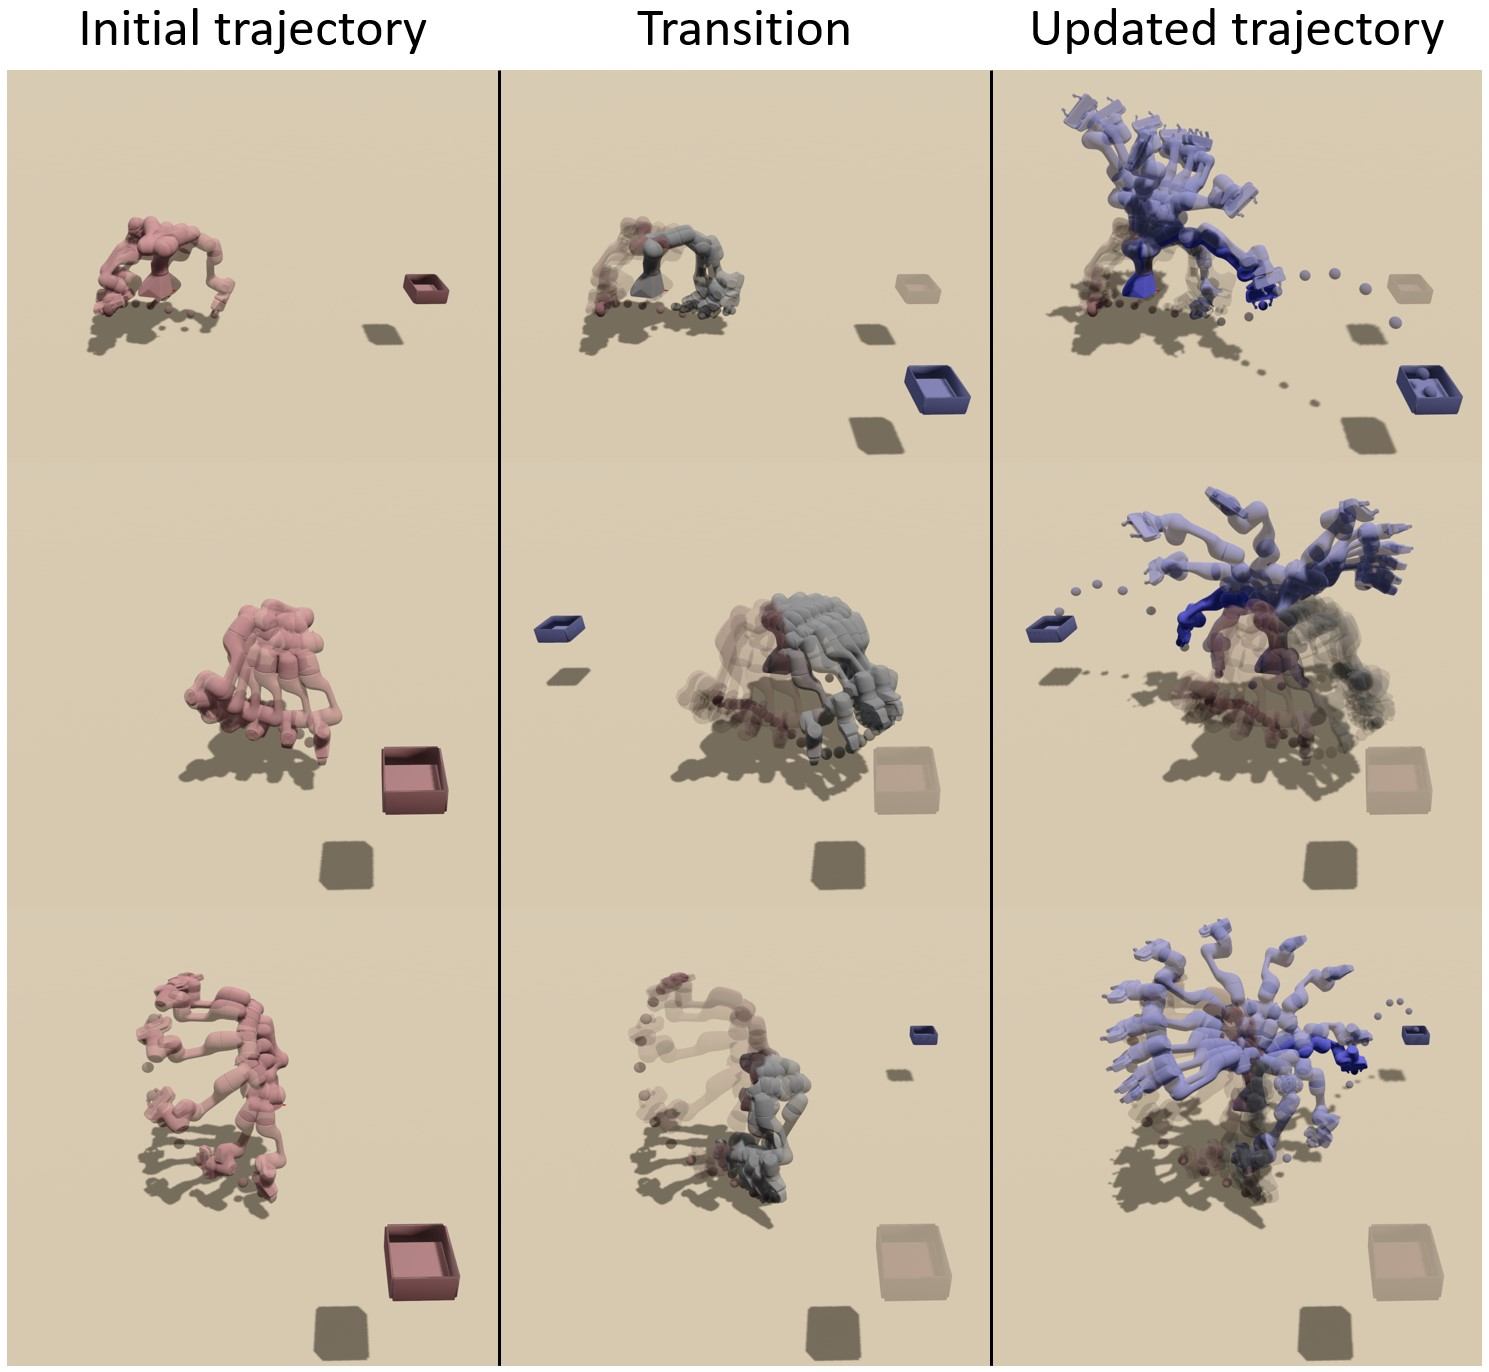
\includegraphics[width=\linewidth]{adaptation.jpg}
    \caption{Online adaptation to changes in target box position: The robot follows an initial trajectory (red), detects a target change, replans an updated trajectory (blue), and executes a transition trajectory (gray) connecting its current phase to the new plan.}
    \label{fig:results3}
\end{figure}

In the replanning step, we sample 100 candidate trajectories $\{(q_i(t),\eta_i)\}_{i=1}^{100}$ conditioned on the new target.  
We then select the trajectory closest to the current configuration $q_c$ by solving
\[
(i^*,t^*) = \arg\min_{i,t}\|q_c-q_i(t)\| \quad \text{s.t. } t<\eta_i.
\]
Next, we construct a transition trajectory from the current phase $(q_c,\dot q_c)$ to $(q_{i^*}(t^*),\dot q_{i^*}(t^*))$ in the selected trajectory, using the following parametric model:
\begin{align}
\label{eq:mp2}
q(t) = &\, q_0 + (q_T-q_0)(3-2s)s^2 
+ \dot q_0 s - (2\dot q_0+\dot q_T)s^2 \nonumber\\
&+ (\dot q_0+\dot q_T)s^3 + s^2(s-1)^2\Phi(s)w,
\end{align}
in a manner analogous to~(\ref{eq:parmetric_model}).
This model enforces $(q_0,\dot q_0)$ at $t=0$ and $(q_T,\dot q_T)$ at $t=T$, and accommodates nonzero boundary velocities.

The transition trajectory must satisfy kinodynamic constraints, which reduces to finding a suitable $w$.  
Empirically, random Gaussian initialization of $w$ often yields at least one valid solution.  
The process is fast enough to run online, enabling the robot to adapt in real time.

Fig.~\ref{fig:results3} illustrates examples: red robots follow the initial plan until the target moves (after 1.8 s), gray robots execute a transition trajectory over $\sim$1 s, and blue robots follow the updated throwing trajectory, completing the throw within 3–5 s depending on target distance.
